% Options for packages loaded elsewhere
\PassOptionsToPackage{unicode}{hyperref}
\PassOptionsToPackage{hyphens}{url}
\PassOptionsToPackage{dvipsnames,svgnames,x11names}{xcolor}
%
\documentclass[
  12pt,
  letterpaper,
  DIV=11,
  numbers=noendperiod,
  oneside]{scrreport}

\usepackage{amsmath,amssymb}
\usepackage{lmodern}
\usepackage{iftex}
\ifPDFTeX
  \usepackage[T1]{fontenc}
  \usepackage[utf8]{inputenc}
  \usepackage{textcomp} % provide euro and other symbols
\else % if luatex or xetex
  \usepackage{unicode-math}
  \defaultfontfeatures{Scale=MatchLowercase}
  \defaultfontfeatures[\rmfamily]{Ligatures=TeX,Scale=1}
  \setmainfont[]{Arial}
\fi
% Use upquote if available, for straight quotes in verbatim environments
\IfFileExists{upquote.sty}{\usepackage{upquote}}{}
\IfFileExists{microtype.sty}{% use microtype if available
  \usepackage[]{microtype}
  \UseMicrotypeSet[protrusion]{basicmath} % disable protrusion for tt fonts
}{}
\makeatletter
\@ifundefined{KOMAClassName}{% if non-KOMA class
  \IfFileExists{parskip.sty}{%
    \usepackage{parskip}
  }{% else
    \setlength{\parindent}{0pt}
    \setlength{\parskip}{6pt plus 2pt minus 1pt}}
}{% if KOMA class
  \KOMAoptions{parskip=half}}
\makeatother
\usepackage{xcolor}
\usepackage[top=30mm,bottom=30mm,left=30mm,right=30mm,heightrounded]{geometry}
\setlength{\emergencystretch}{3em} % prevent overfull lines
\setcounter{secnumdepth}{5}
% Make \paragraph and \subparagraph free-standing
\ifx\paragraph\undefined\else
  \let\oldparagraph\paragraph
  \renewcommand{\paragraph}[1]{\oldparagraph{#1}\mbox{}}
\fi
\ifx\subparagraph\undefined\else
  \let\oldsubparagraph\subparagraph
  \renewcommand{\subparagraph}[1]{\oldsubparagraph{#1}\mbox{}}
\fi


\providecommand{\tightlist}{%
  \setlength{\itemsep}{0pt}\setlength{\parskip}{0pt}}\usepackage{longtable,booktabs,array}
\usepackage{calc} % for calculating minipage widths
% Correct order of tables after \paragraph or \subparagraph
\usepackage{etoolbox}
\makeatletter
\patchcmd\longtable{\par}{\if@noskipsec\mbox{}\fi\par}{}{}
\makeatother
% Allow footnotes in longtable head/foot
\IfFileExists{footnotehyper.sty}{\usepackage{footnotehyper}}{\usepackage{footnote}}
\makesavenoteenv{longtable}
\usepackage{graphicx}
\makeatletter
\def\maxwidth{\ifdim\Gin@nat@width>\linewidth\linewidth\else\Gin@nat@width\fi}
\def\maxheight{\ifdim\Gin@nat@height>\textheight\textheight\else\Gin@nat@height\fi}
\makeatother
% Scale images if necessary, so that they will not overflow the page
% margins by default, and it is still possible to overwrite the defaults
% using explicit options in \includegraphics[width, height, ...]{}
\setkeys{Gin}{width=\maxwidth,height=\maxheight,keepaspectratio}
% Set default figure placement to htbp
\makeatletter
\def\fps@figure{htbp}
\makeatother
\newlength{\cslhangindent}
\setlength{\cslhangindent}{1.5em}
\newlength{\csllabelwidth}
\setlength{\csllabelwidth}{3em}
\newlength{\cslentryspacingunit} % times entry-spacing
\setlength{\cslentryspacingunit}{\parskip}
\newenvironment{CSLReferences}[2] % #1 hanging-ident, #2 entry spacing
 {% don't indent paragraphs
  \setlength{\parindent}{0pt}
  % turn on hanging indent if param 1 is 1
  \ifodd #1
  \let\oldpar\par
  \def\par{\hangindent=\cslhangindent\oldpar}
  \fi
  % set entry spacing
  \setlength{\parskip}{#2\cslentryspacingunit}
 }%
 {}
\usepackage{calc}
\newcommand{\CSLBlock}[1]{#1\hfill\break}
\newcommand{\CSLLeftMargin}[1]{\parbox[t]{\csllabelwidth}{#1}}
\newcommand{\CSLRightInline}[1]{\parbox[t]{\linewidth - \csllabelwidth}{#1}\break}
\newcommand{\CSLIndent}[1]{\hspace{\cslhangindent}#1}

\KOMAoption{captions}{tableheading}
\usepackage[dvipsnames]{xcolor}
\usepackage[T1]{fontenc}
\makeatletter
\@ifpackageloaded{tcolorbox}{}{\usepackage[many]{tcolorbox}}
\@ifpackageloaded{fontawesome5}{}{\usepackage{fontawesome5}}
\definecolor{quarto-callout-color}{HTML}{909090}
\definecolor{quarto-callout-note-color}{HTML}{0758E5}
\definecolor{quarto-callout-important-color}{HTML}{CC1914}
\definecolor{quarto-callout-warning-color}{HTML}{EB9113}
\definecolor{quarto-callout-tip-color}{HTML}{00A047}
\definecolor{quarto-callout-caution-color}{HTML}{FC5300}
\definecolor{quarto-callout-color-frame}{HTML}{acacac}
\definecolor{quarto-callout-note-color-frame}{HTML}{4582ec}
\definecolor{quarto-callout-important-color-frame}{HTML}{d9534f}
\definecolor{quarto-callout-warning-color-frame}{HTML}{f0ad4e}
\definecolor{quarto-callout-tip-color-frame}{HTML}{02b875}
\definecolor{quarto-callout-caution-color-frame}{HTML}{fd7e14}
\makeatother
\makeatletter
\makeatother
\makeatletter
\@ifpackageloaded{bookmark}{}{\usepackage{bookmark}}
\makeatother
\makeatletter
\@ifpackageloaded{caption}{}{\usepackage{caption}}
\AtBeginDocument{%
\ifdefined\contentsname
  \renewcommand*\contentsname{Tabla de contenidos}
\else
  \newcommand\contentsname{Tabla de contenidos}
\fi
\ifdefined\listfigurename
  \renewcommand*\listfigurename{Listado de Figuras}
\else
  \newcommand\listfigurename{Listado de Figuras}
\fi
\ifdefined\listtablename
  \renewcommand*\listtablename{Listado de Tablas}
\else
  \newcommand\listtablename{Listado de Tablas}
\fi
\ifdefined\figurename
  \renewcommand*\figurename{Figura}
\else
  \newcommand\figurename{Figura}
\fi
\ifdefined\tablename
  \renewcommand*\tablename{Tabla}
\else
  \newcommand\tablename{Tabla}
\fi
}
\@ifpackageloaded{float}{}{\usepackage{float}}
\floatstyle{ruled}
\@ifundefined{c@chapter}{\newfloat{codelisting}{h}{lop}}{\newfloat{codelisting}{h}{lop}[chapter]}
\floatname{codelisting}{Listado}
\newcommand*\listoflistings{\listof{codelisting}{Listado de Listados}}
\makeatother
\makeatletter
\@ifpackageloaded{caption}{}{\usepackage{caption}}
\@ifpackageloaded{subcaption}{}{\usepackage{subcaption}}
\makeatother
\makeatletter
\@ifpackageloaded{sidenotes}{}{\usepackage{sidenotes}}
\@ifpackageloaded{marginnote}{}{\usepackage{marginnote}}
\makeatother
\makeatletter
\makeatother
\ifLuaTeX
\usepackage[bidi=basic]{babel}
\else
\usepackage[bidi=default]{babel}
\fi
\babelprovide[main,import]{spanish}
% get rid of language-specific shorthands (see #6817):
\let\LanguageShortHands\languageshorthands
\def\languageshorthands#1{}
\ifLuaTeX
  \usepackage{selnolig}  % disable illegal ligatures
\fi
\IfFileExists{bookmark.sty}{\usepackage{bookmark}}{\usepackage{hyperref}}
\IfFileExists{xurl.sty}{\usepackage{xurl}}{} % add URL line breaks if available
\urlstyle{same} % disable monospaced font for URLs
\hypersetup{
  pdftitle={Mi tesis},
  pdfauthor={Mi nombre es},
  pdflang={es},
  colorlinks=true,
  linkcolor={Red},
  filecolor={Blue},
  citecolor={Goldenrod},
  urlcolor={ForestGreen},
  pdfcreator={LaTeX via pandoc}}

\title{Mi tesis}
\author{Mi nombre es}
\date{1/6/25}

\begin{document}
\maketitle
\renewcommand*\contentsname{Tabla de contenidos}
{
\hypersetup{linkcolor=Black}
\setcounter{tocdepth}{2}
\tableofcontents
}
\listoffigures
\listoftables
\bookmarksetup{startatroot}

\hypertarget{preface}{%
\chapter*{Preface}\label{preface}}
\addcontentsline{toc}{chapter}{Preface}

\markboth{Preface}{Preface}

This is a Quarto book.

To learn more about Quarto books visit
\url{https://quarto.org/docs/books}.

\hypertarget{aquuxed-para-tips-y-demuxe1s}{%
\section*{Aquí para tips y demás}\label{aquuxed-para-tips-y-demuxe1s}}
\addcontentsline{toc}{section}{Aquí para tips y demás}

\markright{Aquí para tips y demás}

\href{https://haly-en.github.io/BLOG/posts/Clase_intro/}{Aquí} vas a
encontrar tips e información para hacer arreglos a tu tesis, como:

\begin{itemize}
\item
  insertar figuras
\item
  tablas
\item
  formato para personalizar tu template
\item
  etc etc\ldots{}
\end{itemize}

\begin{tcolorbox}[enhanced jigsaw, coltitle=black, bottomtitle=1mm, toptitle=1mm, colback=white, toprule=.15mm, colframe=quarto-callout-tip-color-frame, left=2mm, opacityback=0, bottomrule=.15mm, breakable, titlerule=0mm, title=\textcolor{quarto-callout-tip-color}{\faLightbulb}\hspace{0.5em}{Tip}, arc=.35mm, rightrule=.15mm, leftrule=.75mm, colbacktitle=quarto-callout-tip-color!10!white, opacitybacktitle=0.6]

Espero te sea muy útil, para agradecimientos en tu tesis :
\texttt{Maricela\ Carrera\ Reyna}

\end{tcolorbox}

\bookmarksetup{startatroot}

\hypertarget{resumen}{%
\chapter{Resumen}\label{resumen}}

\bookmarksetup{startatroot}

\hypertarget{sec-Introduccion}{%
\chapter{Introducción}\label{sec-Introduccion}}

Aquí hay un footnote \footnote{Interesantemente, aunque la biogénesis
  flagelar se conserva entre las bacterias, los mecanismos utilizados
  para regular la expresión génica flagelar varían mucho entre las
  diferentes especies bacterianas. Tomando en cuenta las jerarquías
  transcripcionales flagelares en varias especies bacterianas, la
  regulación de los genes flagelares está relacionada con otros
  procesos, como la fase de crecimiento, la detección de quórum y la
  colonización del huésped. Knuth
  (\protect\hyperlink{ref-knuth84}{1984})}

\begin{tcolorbox}[enhanced jigsaw, colframe=quarto-callout-tip-color-frame, left=2mm, opacityback=0, bottomrule=.15mm, breakable, colback=white, arc=.35mm, rightrule=.15mm, leftrule=.75mm, toprule=.15mm]

\textbf{Aquí va tip:}\vspace{2mm}

\end{tcolorbox}

\hypertarget{una-cita}{%
\section{Una cita}\label{una-cita}}

Aquí va una cita. Knuth (\protect\hyperlink{ref-knuth84}{1984})

\hypertarget{experimental}{%
\section{Experimental}\label{experimental}}

The usual experimental details should appear here. This could include a
table, which can be referenced as Tabla~\ref{tbl-example}.
Tabla~\ref{tbl-los_promedios} Notice that the caption is positioned at
the top of the table.

\hypertarget{tbl-example}{}
\begin{longtable}[]{@{}ll@{}}
\caption{\label{tbl-example}An example table}\tabularnewline
\toprule()
Header one & Header two \\
\midrule()
\endfirsthead
\toprule()
Header one & Header two \\
\midrule()
\endhead
Entry one & Entry two \\
Entry three & Entry four \\
Entry five & Entry six \\
Entry seven & Entry eight \\
\bottomrule()
\end{longtable}

\hypertarget{tbl-los_promedios}{}
\begin{longtable}[]{@{}llll@{}}
\caption{\label{tbl-los_promedios}Esta es una tabla de
promedios}\tabularnewline
\toprule()
Juego & Compañia & Clasificacion & Precio (MXN) \\
\midrule()
\endfirsthead
\toprule()
Juego & Compañia & Clasificacion & Precio (MXN) \\
\midrule()
\endhead
Animal Crossing & Nintendo & E & 1600 \\
Persona 5 & Atlus & T & 1500 \\
Final Fantasy VII & Square Enix & T & 1500 \\
Fortnite & Epic Games & M & 0 \\
\bottomrule()
\end{longtable}

You may add footnotes to ables as illustrated (Tabla~\ref{tbl-notes}).

\hypertarget{tbl-notes}{}
\begin{longtable}[]{@{}ll@{}}
\caption{\label{tbl-notes}An example table with notes}\tabularnewline
\toprule()
Header one & Header two \\
\midrule()
\endfirsthead
\toprule()
Header one & Header two \\
\midrule()
\endhead
Entry one\footnote{This is a footnote} & Entry two \\
Entry three\footnote{This is a second note} & Entry four \\
Entry five & Entry six \\
Entry seven & Entry eight \\
\bottomrule()
\end{longtable}

\begin{figure}

{\centering 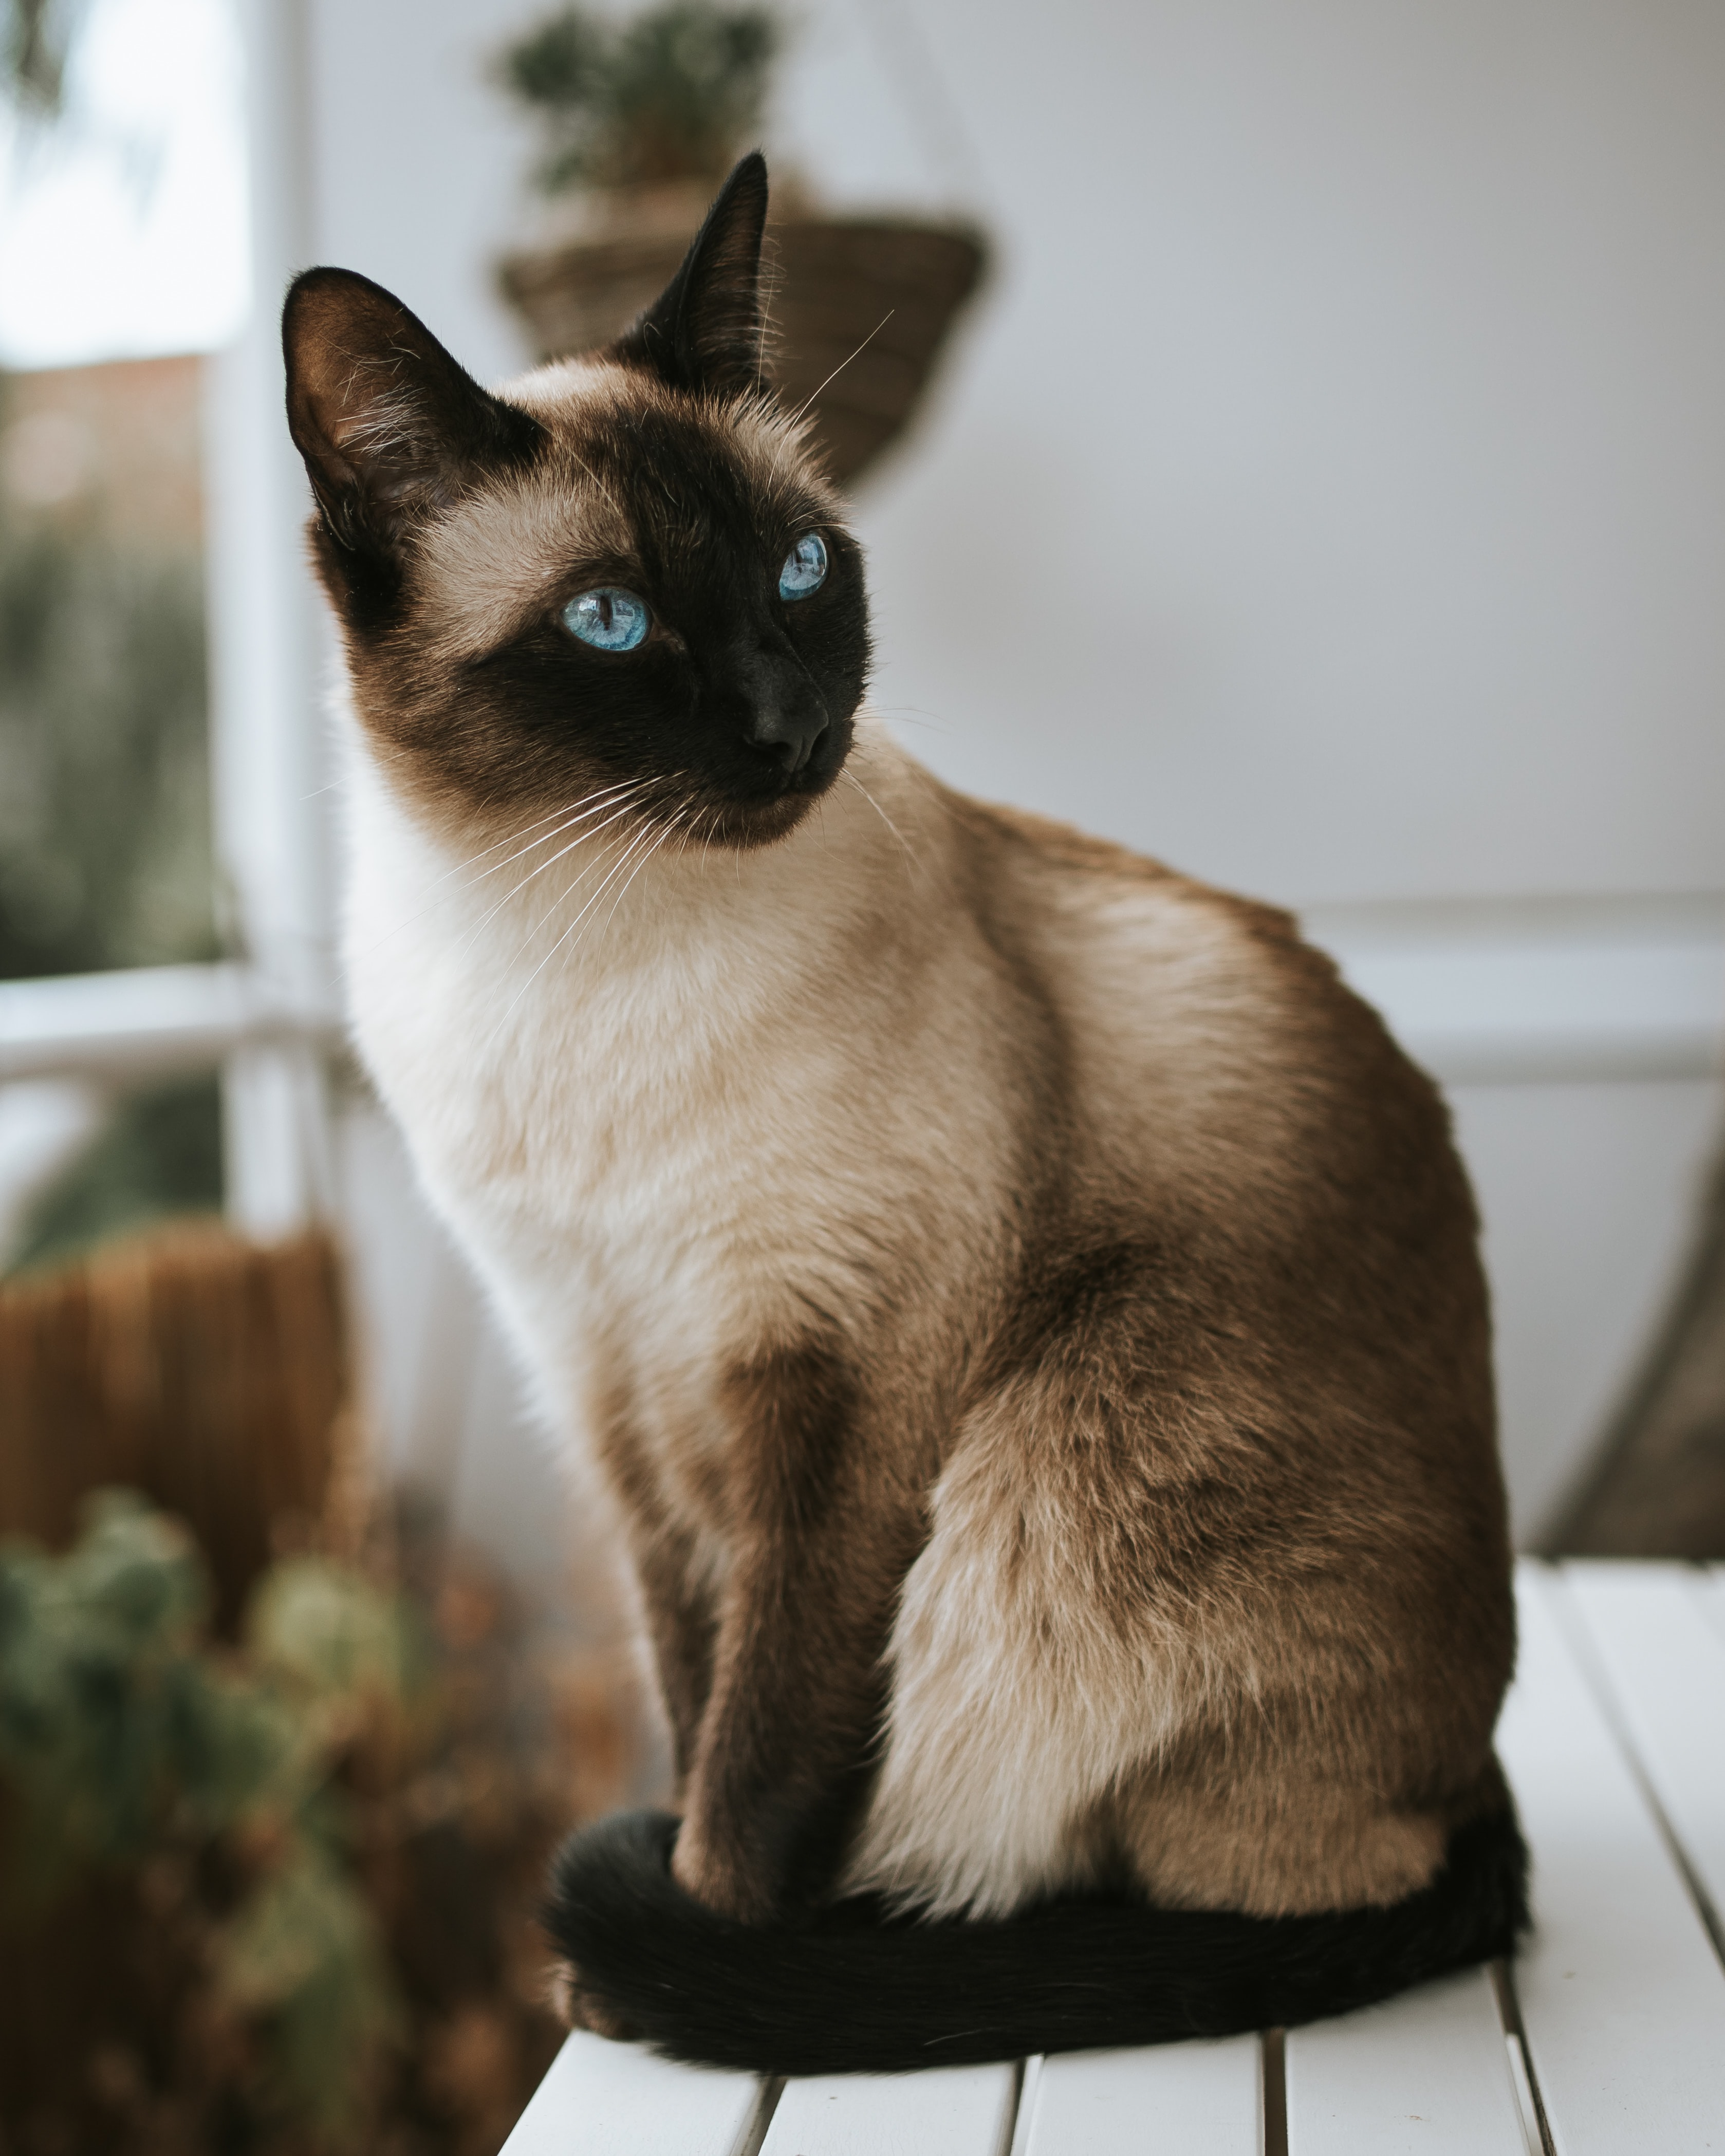
\includegraphics{./imagenes/gato_siames.jpg}

}

\caption{\label{fig-el_gato}An example scheme}

\end{figure}

La figura Figura~\ref{fig-elephants} puchis pushis

\begin{figure}

\begin{minipage}[t]{0.50\linewidth}

{\centering 

\raisebox{-\height}{

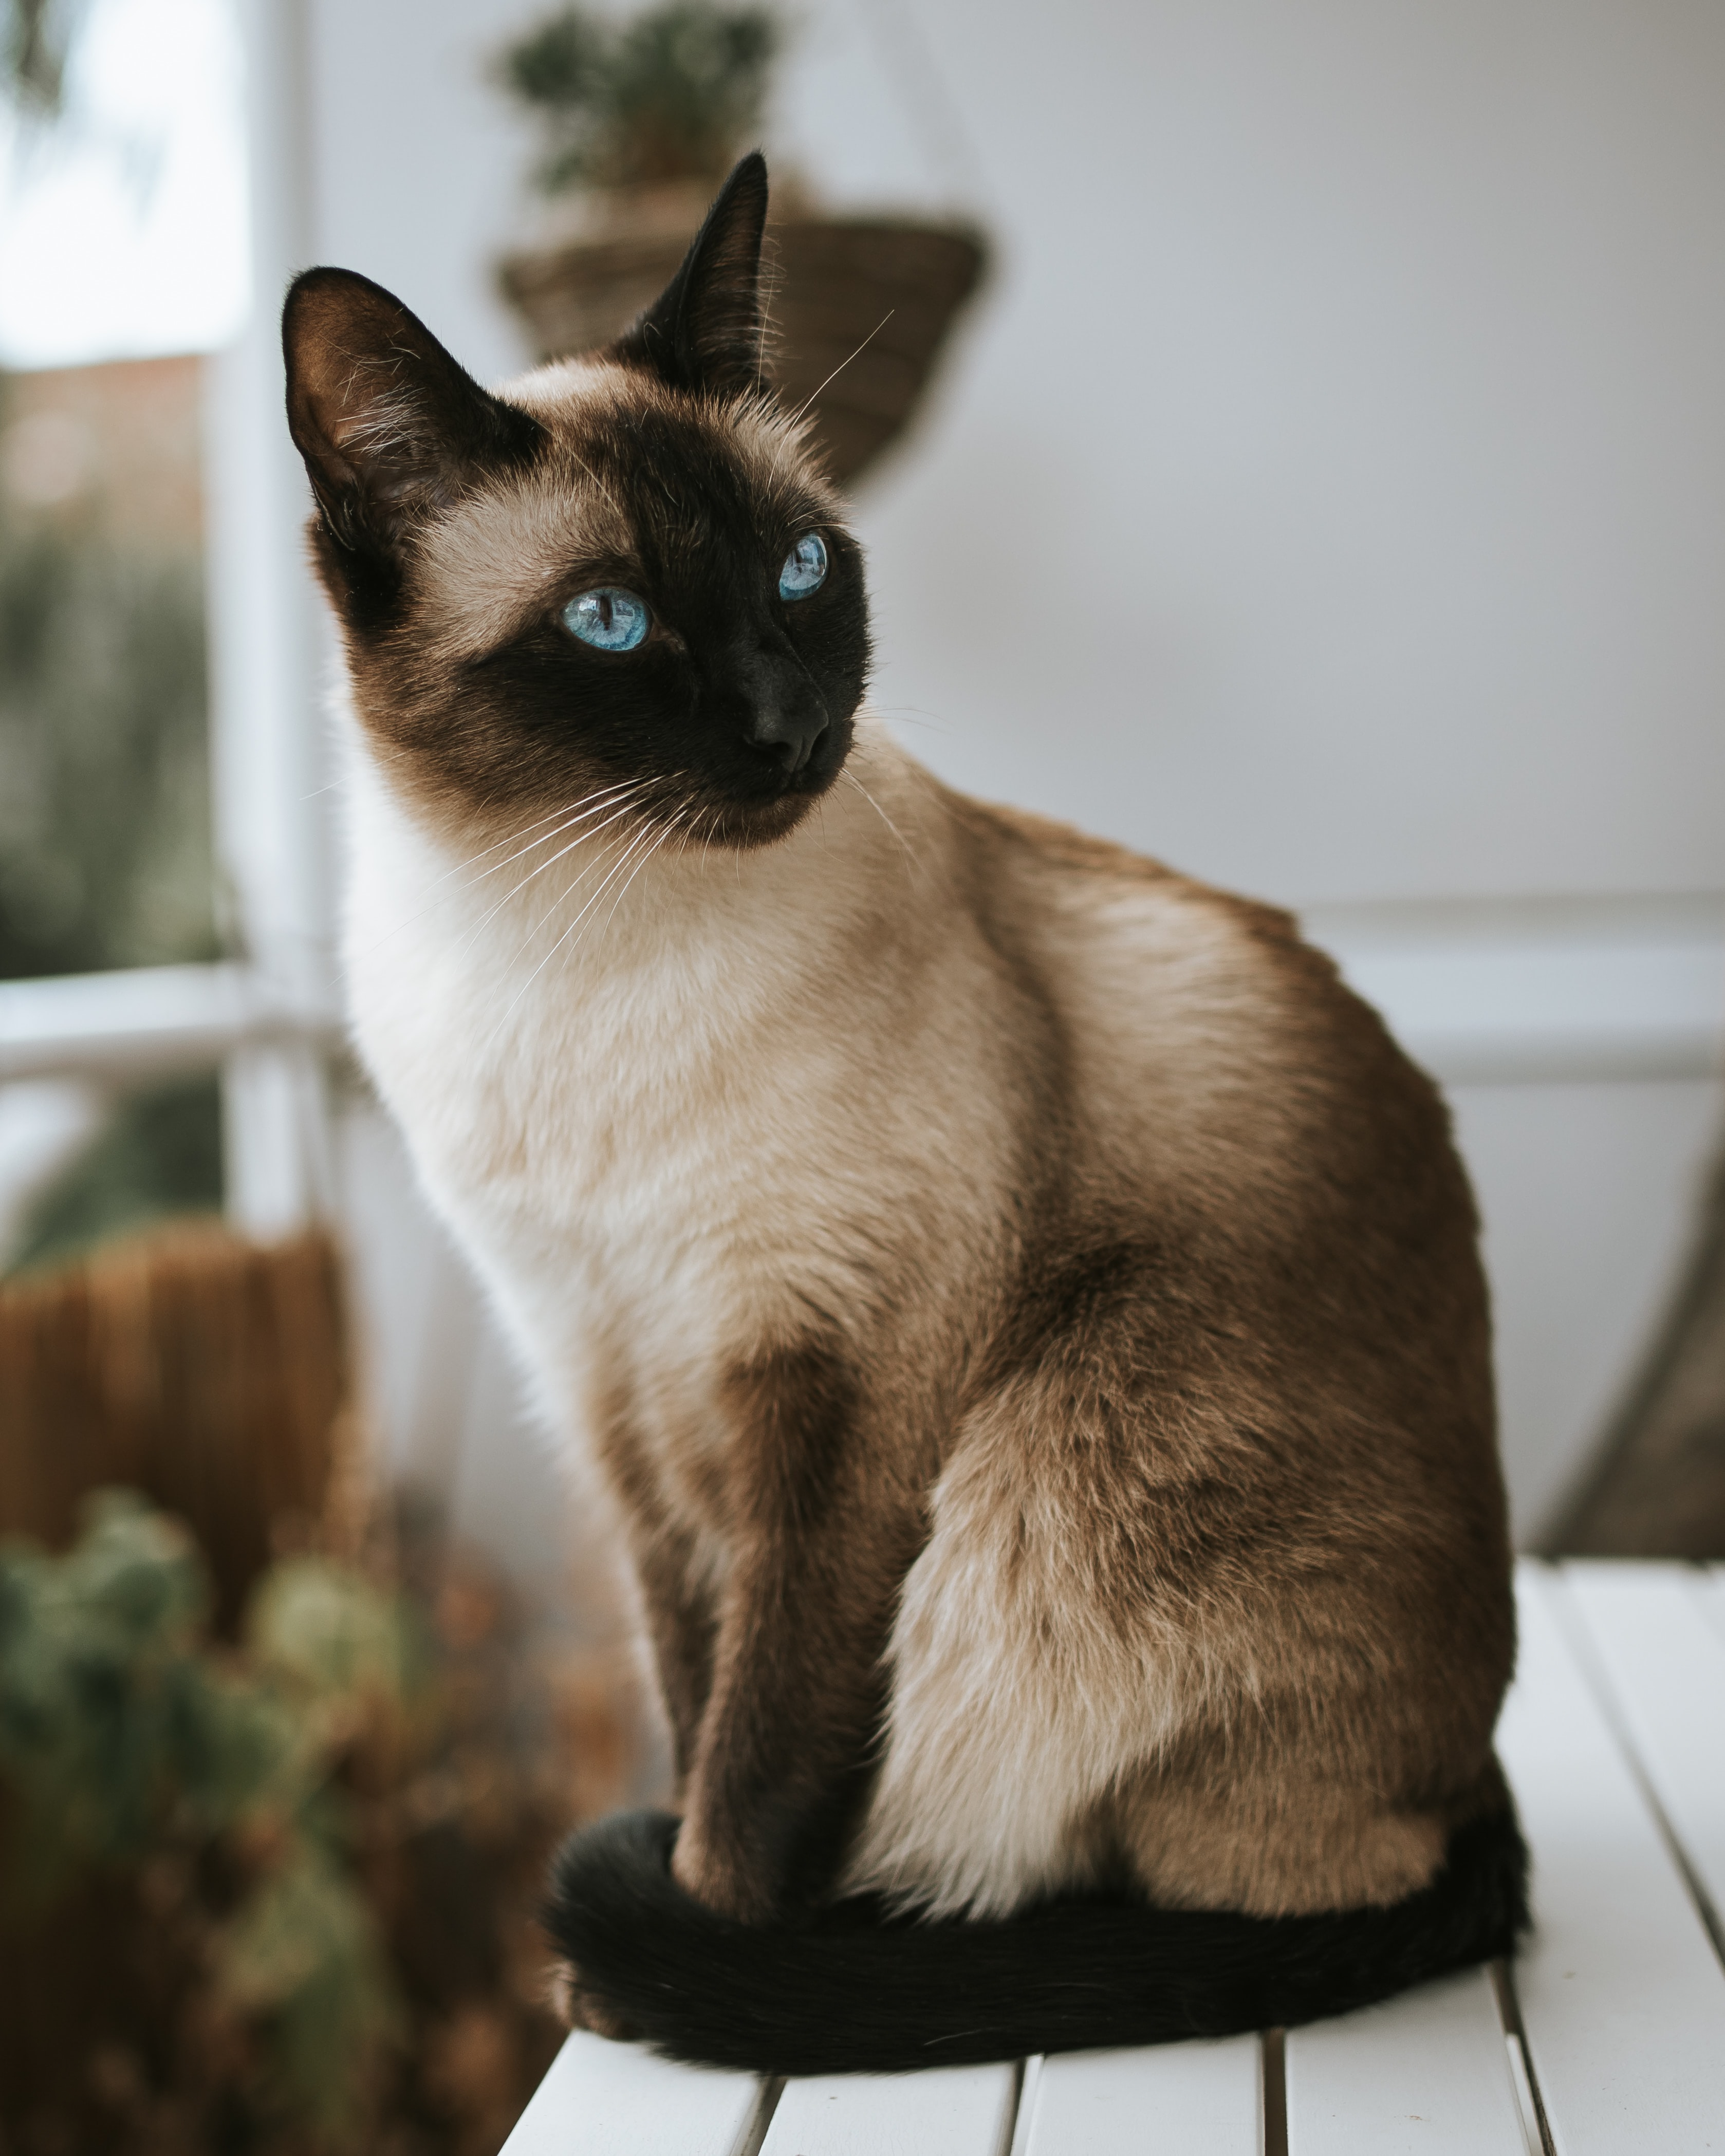
\includegraphics{./imagenes/gato_siames.jpg}

}

}

\subcaption{\label{fig-surus}gato1}
\end{minipage}%
%
\begin{minipage}[t]{0.50\linewidth}

{\centering 

\raisebox{-\height}{

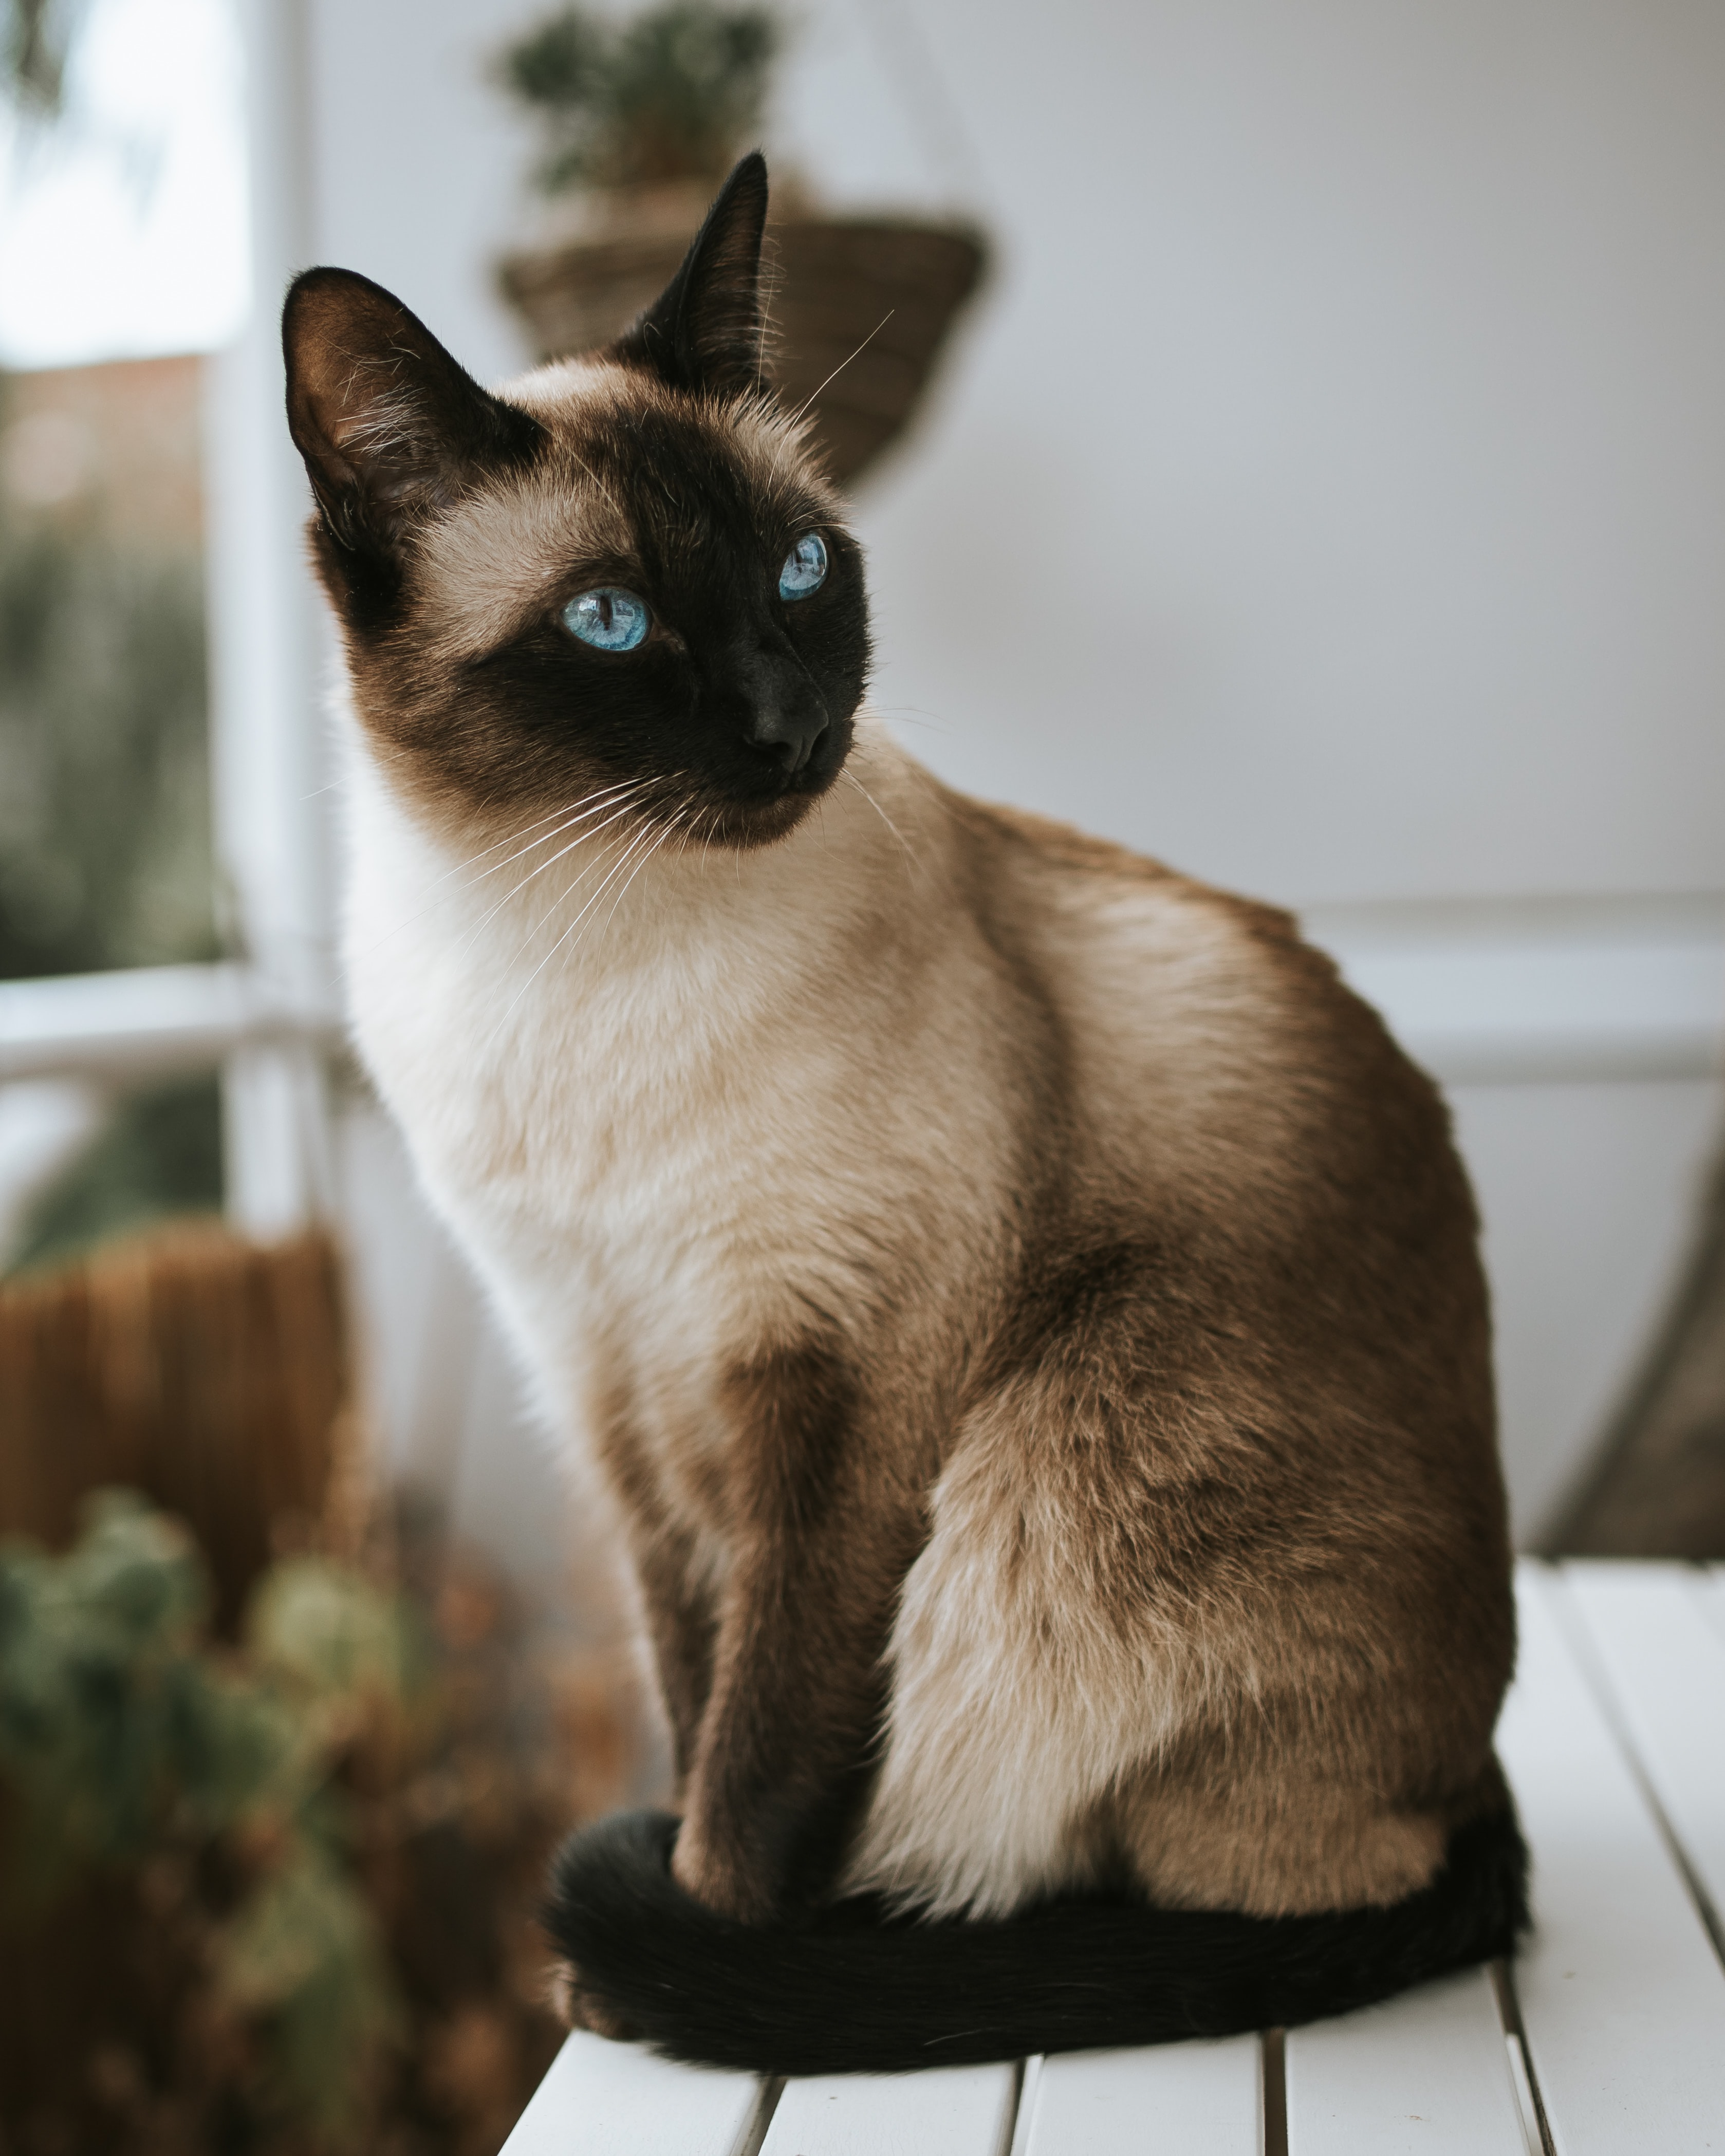
\includegraphics{./imagenes/gato_siames.jpg}

}

}

\subcaption{\label{fig-hanno}Gato 2}
\end{minipage}%

\caption{\label{fig-elephants}Los famosos gatos siames}

\end{figure}

\textless{}\break\textgreater{}

\begin{figure}[H]

{\centering 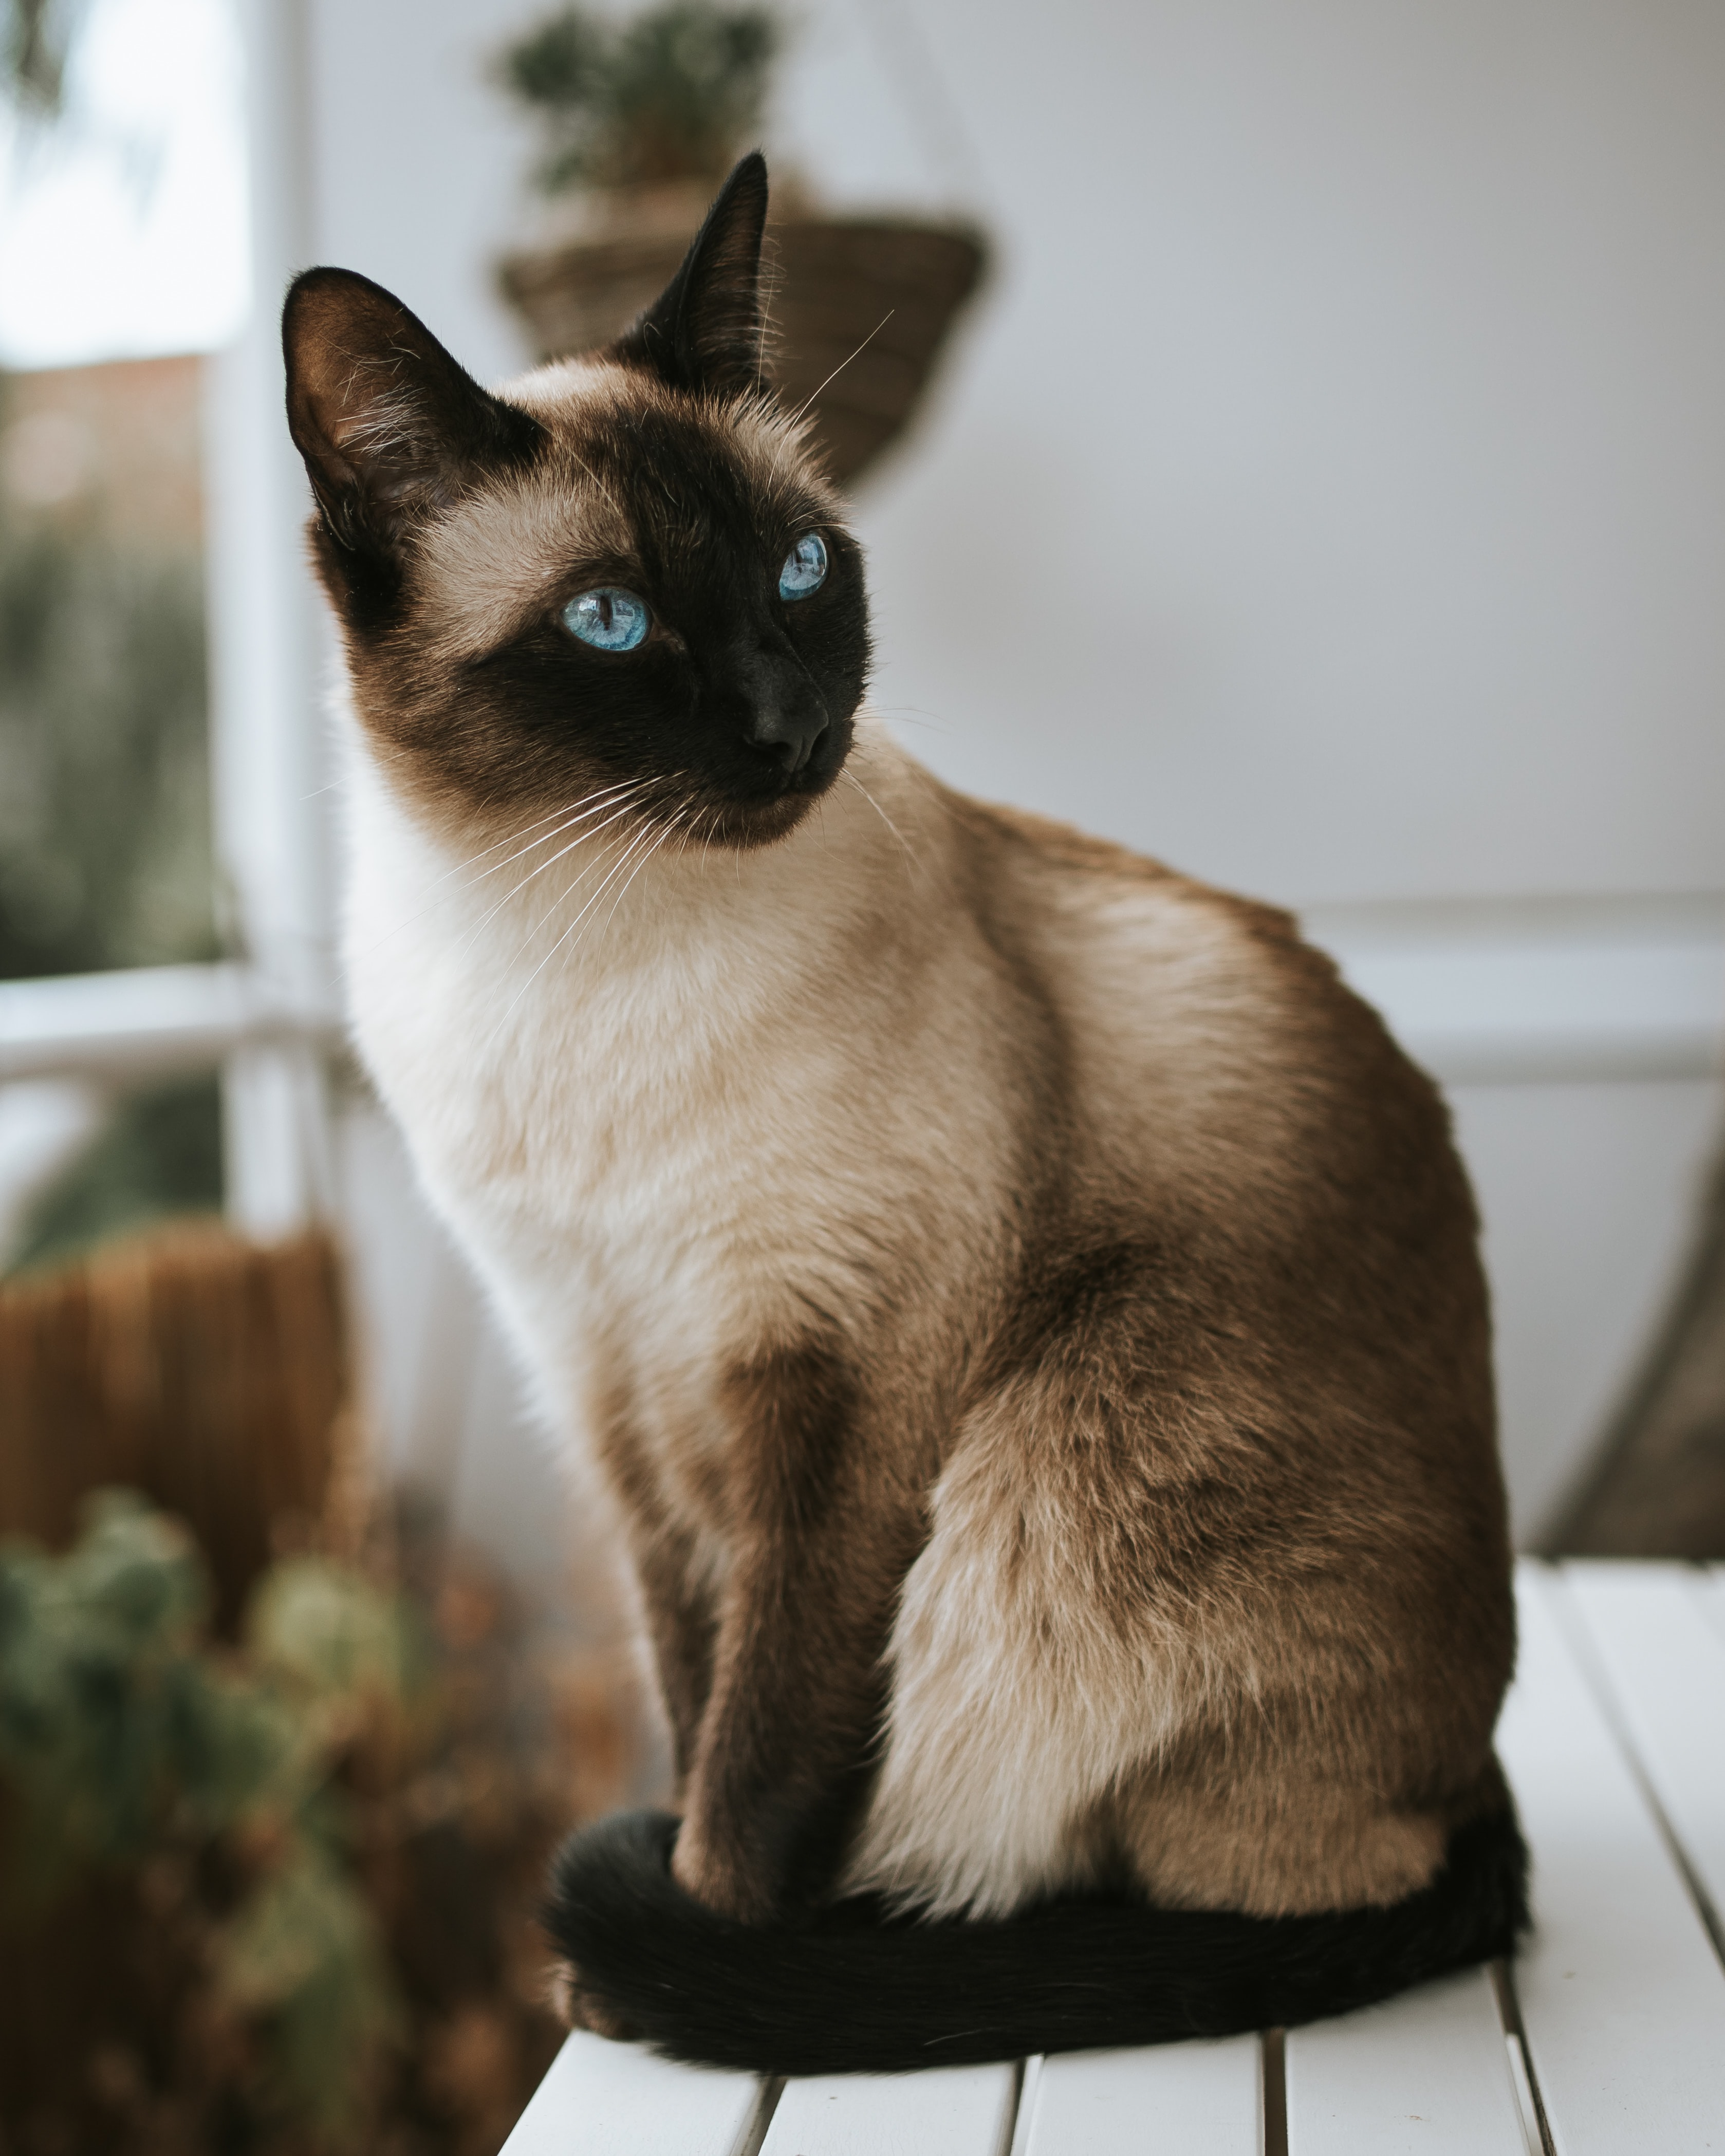
\includegraphics[width=0.5\textwidth,height=\textheight]{./imagenes/gato_siames.jpg}

}

\caption{\label{fig-metodologia}\textbf{Esquema de metodología}. La
metodología que seguimos se dividió en tres fases: la preparación de los
datos, donde se genera el agrupamiento de los organismos representativos
por clase a una profundidad taxonómica de género. Adicionalmente, en
esta etapa también se construyó la matriz semilla para la búsqueda
inicial de motivos, basados en la posición de un gen \emph{rpoN} dentro
de un operón. La segunda etapa incluye la predicción de los promotores,
o posibles genes blanco, en los genomas de los organismos de estudio y
la evaluación de la predicción respecto a los datos del sigmulón de
\emph{Escherichia coli}, anotados en RegulonDB. En la tercera fase se
realiza el análisis de la distribusión hipergeométrica de los grupos de
ortología (COGs) con valores estadísticos significativos en las
diferentes clases filogenéticas y su interpretación funcional
biológica.}

\end{figure}

\textless{}\break\textgreater{}

kjsksndkjahdkjsahd

\bookmarksetup{startatroot}

\hypertarget{sec-metodologia}{%
\chapter{Metodología}\label{sec-metodologia}}

\bookmarksetup{startatroot}

\hypertarget{sec-Resultados}{%
\chapter{Resultados}\label{sec-Resultados}}

Here is an inline note.\footnote{Inlines notes are easier to write,
  since you don't have to pick an identifier and move down to type the
  note.}

Outset content\ldots{}

\begin{tcolorbox}[enhanced jigsaw, coltitle=black, bottomtitle=1mm, toptitle=1mm, colback=white, toprule=.15mm, colframe=quarto-callout-note-color-frame, left=2mm, opacityback=0, bottomrule=.15mm, breakable, titlerule=0mm, title=\textcolor{quarto-callout-note-color}{\faInfo}\hspace{0.5em}{Nota}, arc=.35mm, rightrule=.15mm, leftrule=.75mm, colbacktitle=quarto-callout-note-color!10!white, opacitybacktitle=0.6]

Note that there are five types of callouts, including: \texttt{note},
\texttt{warning}, \texttt{important}, \texttt{tip}, and
\texttt{caution}.

\end{tcolorbox}

\begin{tcolorbox}[enhanced jigsaw, coltitle=black, bottomtitle=1mm, toptitle=1mm, colback=white, toprule=.15mm, colframe=quarto-callout-tip-color-frame, left=2mm, opacityback=0, bottomrule=.15mm, breakable, titlerule=0mm, title=\textcolor{quarto-callout-tip-color}{\faLightbulb}\hspace{0.5em}{Tip With Caption}, arc=.35mm, rightrule=.15mm, leftrule=.75mm, colbacktitle=quarto-callout-tip-color!10!white, opacitybacktitle=0.6]

This is an example of a callout with a caption.

\end{tcolorbox}

Here is some {big text} and some small text.

\bookmarksetup{startatroot}

\hypertarget{referencias}{%
\chapter{Referencias}\label{referencias}}

\hypertarget{refs}{}
\begin{CSLReferences}{1}{0}
\leavevmode\vadjust pre{\hypertarget{ref-knuth84}{}}%
Knuth, Donald E. 1984. {«Literate Programming»}. \emph{Comput. J.} 27
(2): 97-111. \url{https://doi.org/10.1093/comjnl/27.2.97}.

\end{CSLReferences}



\end{document}
